\documentclass{article}

\usepackage{todonotes}
\usepackage{xspace}
\usepackage{url}
\usepackage{alltt}
\usepackage{geometry}
\usepackage{enumitem}   
\geometry{a4paper, margin=1in}


\newcommand{\contractlarva}{\textsc{contractLarva}\xspace}
\newcommand{\keyword}[1]{\textit{$\langle$#1$\rangle$}}
\newcommand{\tildearrow}{{\raise.37ex\hbox{$\scriptstyle\mathtt{\sim}$}}>\xspace}

\begin{document}
\title{\contractlarva v0.2$\alpha$\\User Manual}
\author{Gordon J. Pace and Joshua Ellul and Shaun Azzopardi\\\texttt{\{gordon.pace|joshua.ellul|shaun.azzopardi\}@um.edu.mt}}
\date{5 December 2017, updated 11 October 2019}
\maketitle


\begin{center}
  \begin{tabular}{|lll|}\hline\qquad&&\qquad\\
    &\begin{minipage}{0.8\textwidth}
      \emph{This is an alpha version of \contractlarva. If you are using the tool on smart contracts which will be deployed on Ethereum, it is recommended that you inspect the code created by the tool before deployment. The authors accept no responsibility of any losses, direct or otherwise, incurred due to the use of the tool.}
    \end{minipage}&\\&&\\
  \hline\end{tabular} 
\end{center}



  \section{Overview}
  
  The notion of smart contracts has enabled anyone to write code which handles potentially large volumes of digital assets, typically in the form of a cryptocurrency. The price to pay for the ease in which this can now be achieved is that many smart contracts are written without necessary safeguards to ensure that they work as envisaged and do not  malfunction. In addition, the language adopted to express such smart contracts on a number of distributed ledger systems has been designed to be Turing-complete --- a language powerful enough able to express any computation. But with power comes responsibility, since more complex computations are more likely to have a higher incidence of bugs. 

  In order to ensure the correct behaviour of a smart contract, one would want to write a specification of what it should be performing, and ensure that it behaves accordingly. In contrast to the implementation, which specifies \emph{how} to calculate the result, the specification only specifies properties which the system behaviour and results should satisfy. While a smart contract implementing a complex voting system might explain how voting, vote delegation, vote weights, etc. work, a property might simply specify that from the moment an issue is put to the vote and the moment a decision is taken, the total number of votes in the system (counting both cast and uncast) will not change. Another property might state that no one will lose their vote unless they invoke a method to delegate it. Similarly, in a wallet management smart contract, one might specify properties such as that a wallet may not change ownership, or that a wallet cannot be initialised more than once. Such properties are typically far easier to state than it is to program a system which satisfies them. Such specifications can be used in various ways e.g. as oracles in testing or as properties for static analysis. Another use is in runtime verification, where the runtime behaviour of the system is compared to the specification in order to identify violations as soon as they happen.

  \contractlarva is a runtime verification tool for smart contracts written in Solidity. The tool takes a specification using dynamic event automata (see Section~\ref{s:deas}) and a Solidity contract, and produces a new Solidity contract which acts just like the original smart contract, but in addition checks the dynamic (runtime) behaviour against the specification, allowing for reparations to be performed in case of a violation.

 One of the challenges in the case of smart contracts lies in what to do if a violation does occur. The tool allows for the person writing the specification to decide how to react to violations. At a simplest level, one can, for instance, block the smart contract from executing further (other than emptying its content).  However, one may also use a more sophisticated approach. For instance, in Section~\ref{s:example} we show an example of specification reparation based on a stake-placing design pattern, in which any party that can potentially violate the contract pays in a stake before running the contract, which will be given to the aggrieved party in case of a violation, but returned to the original owner if the contract terminates without violations. 
 
 \contractlarva is a tool still in active development and planned to be extended in the future, with some planned extensions being listed in Section~\ref{s:extensions}. However, the tool is being released as open source to encourage independent extensions and offshoots to the tool.

  \section{Specifying Properties using Dynamic Event Automata}
  \label{s:deas}

  In order to specify properties, \contractlarva used \emph{dynamic event automata} (DEA) --- an automaton-based formalism, based on that used in the Larva runtime verification tool for Java\footnote{\url{http://www.cs.um.edu.mt/svrg/Tools/LARVA}}. 
  
Such specifications monitor for events (the choice of the term \emph{event} is unfortunately overloaded with the notion of events in Solidity --- in \contractlarva, the use of the term is limited to the notion of event triggers as used in DEAs unless explicitly otherwise noted) over the contract and enable the specification of event traces which are not desirable. The tool allows capturing two types of events: (i) control-flow events corresponding to entry and exit points of functions defined in the smart contract, written \texttt{before(f)} and \texttt{after(f)} to refer to the entry and exit point of function \texttt{f} respectively; and (ii) data-flow events corresponding to changes in values of variables, written as \texttt{v@e} to denote the event when variable \texttt{v} is changed and expression \texttt{e} (which can also refer to the previous value of \texttt{v} as \texttt{LARVA\_previous\_v}) holds e.g. \texttt{winout@(winout < LARVA\_previous\_winout)} identifies points in the execution of the contract when the win-out amount is decreased. 

At their most basic level, our specifications will be expressed as (deterministic) automata, listening to contract event triggers. States annotated with a cross denote that a violation has occurred. For instance, consider a smart contract which allows for its initiator to open the gambling table (\texttt{openTable}), on which other users may place a wager (\texttt{placeWager}), and then resolve it (\texttt{resolveWager}) any number of times. The table creator may close down a table (\texttt{closeTable}) as long as it has no unresolved wagers. The automaton shown in Fig.~\ref{f:specifications}(a) ensures that a violation is identified if the table is closed when a wager has been placed but not resolved.

\begin{figure} 
\centerline{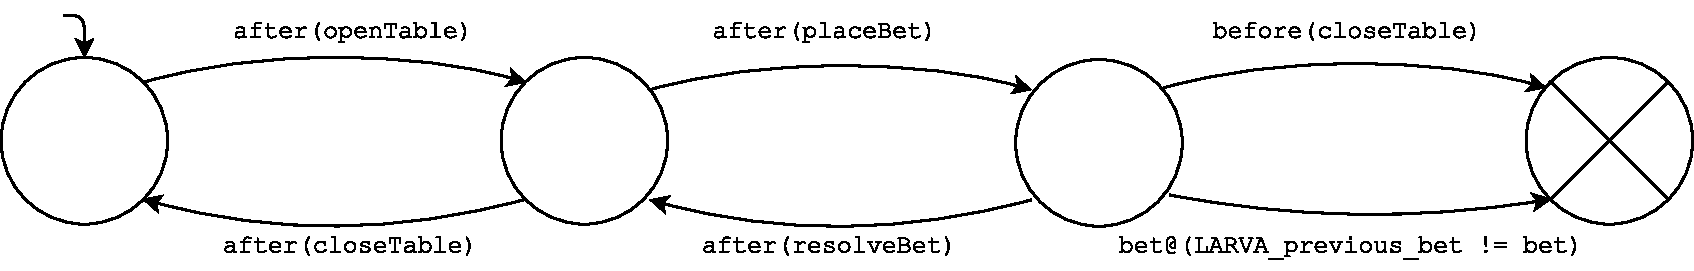
\includegraphics[scale=0.5]{images/example-1.pdf}}
\bigskip
\centerline{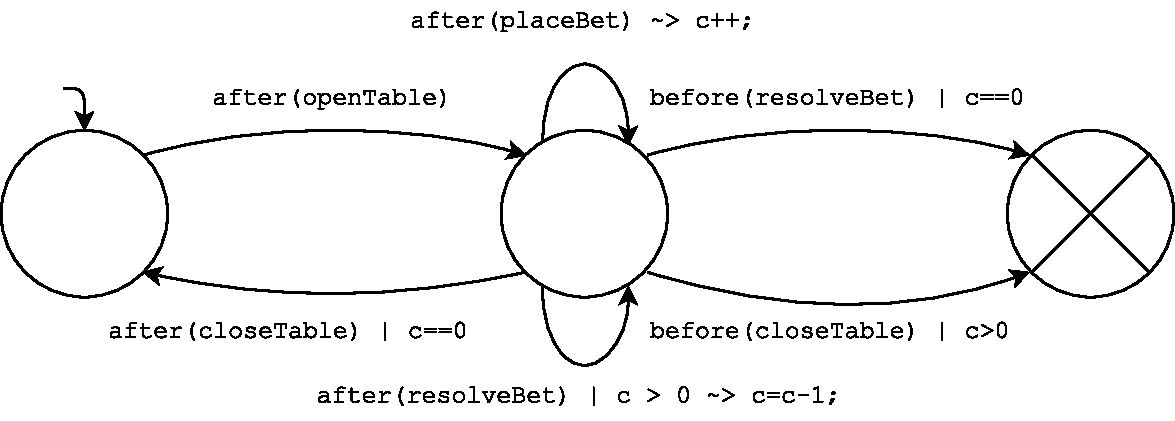
\includegraphics[scale=0.5]{images/example-2.pdf}}
%\medskip
%\centerline{\includegraphics[scale=0.125]{images/example-3.png}}
\caption{Contract specification examples (a) a betting table may not be closed when there is a placed wager which has not been resolved; (b) generalisation of the previous specification to allow for multiple simultaneous wages to be placed on the table.}
\label{f:specifications}
\end{figure}

The automata used are, however, symbolic automata --- in that they may use and manipulate variables. Transitions are annotated by a triple: \texttt{e | c $\sim$> a}, where \texttt{e} is the event which will trigger the transition, \texttt{c} is a condition over the state of the contract (and additional contract property variables) determining whether the transition is to be taken, and finally \texttt{a} is an executable action (code) which will be executed if the transition is taken. Fig.~\ref{f:specifications}(b) is a generalisation of the previous property, to handle the case when multiple wagers may be simultaneously placed and resolved on the same table. The actions typically impact just a number of variables local to the monitors (i.e. not the state of the system itself), although in some cases, however, specifically in the case of a property violation, one may choose to change the system state in order to make up for violated invariants.

%Finally, we note that in a smart contract one can have a notion of multiple instances of a (conceptual) object, for each of which a property is expected to hold. For instance, in the previous example, one may want to monitor the property independently for each table opened. Although this can be encoded with symbolic automata, the resulting specification will be unnecessarily complex. In order to handle such specifications more effectively, we have a notion of replication --- we can annotate a specification automaton as a replicated one by identifying which event creates a new instance of the property and how one can identify which instance a particular event corresponds to. Fig.~\ref{f:specifications}(c) shows how the the previous property can be replicated for each table. We also use acceptance states (marked using a double circle) to denote when the specification can no longer be violated.
%


  \section{Tool Syntax}
  The tool \contractlarva allows the specification of properties using DEAs over method calls and setting of global variables in a smart contract written in Solidity. In addition, the tool allows for the specification of what happens when a specification is violated.
  
  \subsection{Properties}
  Each property in a \contractlarva specification file is written in the form of a DEA as described in the previous section. The top level structure of a DEA is as follows:
  
  \small\begin{alltt}
  DEA \keyword{PropertyName} \{
    states \{
      \ldots
    \}
    transitions \{
      \ldots
    \}
  \}
  \end{alltt}\normalsize
 
  The property name is simply an identifier to be able to refer to the DEA by name. States are declared in the \texttt{states} block of the script, and are written as a semi-colon terminated sequence. Initial, bad and accepting states can be tagged by following the state name by a colon and the type of the state. There can only be one initial state, but multiple bad and accepting states are possible. For example, the states of a four state DEA can declared as follows:

  \small\begin{alltt}
    states \{
      TableOpen: initial;
      TableClosed: accept;
      CasinoClosed: accept;
      BetPlaced;
      PotReduced: bad;
    \}
  \end{alltt}\normalsize

  Transitions are also written as a semicolon terminated sequence, where each transitions is written as: \texttt{src -[label]-> dst}, where (i) \texttt{src} is the name of the source state of the transition, (ii) \texttt{dst} is the destination state, and (iii) \texttt{label} is the guarded event on the transition.
  
  The syntax for labels is as follows: \texttt{event | guard \tildearrow action}, where (i) \texttt{event} is the trigger of the transition, (ii) \texttt{guard} is a Solidity expression which will be evaluated to decide whether or not to take the transition; and (iii) \texttt{action} is a Solidity statement (or block) which will be executed if the transition is taken. Both the condition and action can be left out, in which case, one can also leave out the separators: for instance \texttt{e | c \tildearrow} can be written as \texttt{e | c} while \texttt{e | \tildearrow a} can be written as \texttt{e \tildearrow a} and \texttt{e | \tildearrow} simply as \texttt{e}.
  
  \noindent There are two types of event triggers which can be used in \contractlarva:
  \begin{enumerate}[label=(\roman*)]
    \item \emph{Control-flow triggers} which trigger when a function is called or returns a value: (a) \texttt{before(function)}, triggers whenever \texttt{function} is called and before any of its code is executed\footnote{The checks and the code are instrumented as a modifier triggering before the function body is executed.}; and  (b) \texttt{after(function)}, triggers the moment \texttt{function} terminates successfully (i.e. not reverted). In both cases, if you want to read the value of the parameters, they can be specified in the event e.g. \texttt{before(payAmount(value))} can be written to have a condition dependent on the parameter. Parameters may be left out altogether if you do not wish to access them e.g.  \texttt{before(payAmount)}.
    \item \emph{Data-flow triggers}, trigger when an assignment on a global variable occurs (even if the value of the variable does not change) --- \texttt{var@(condition)}  triggers whenever variable \texttt{var} is assigned to (just after the assignment is performed), with the \texttt{condition} holding. The condition is optional, in which case any assignment to the variable will trigger the event. Furthermore, the condition in variable assignment triggers can refer the value of variable \texttt{var} before the assignment using the syntax \texttt{LARVA\_previous\_var} e.g. to trigger when a variable \texttt{x} is assigned to a larger value, one would use the event \texttt{x@(x > LARVA\_previous\_x)}.
  \end{enumerate}
      
  \noindent The following is an example of a complete DEA property, using a global variable \texttt{total} to keep count of the running total of bets (we will see how to declare such variables in the script in the next section):
  
  \small\begin{alltt}
  DEA NoReduction \{
    states \{
      TableOpen: initial;
      TableClosed: accept;
      BetPlaced;
      PotReduced: bad;
    \}
    transitions \{
      TableOpen -[after(closeTable) | pot == 0 ]-> TableClosed;
      TableOpen 
        -[after(placeBet(\_value)) | \_value <= pot \tildearrow total += \_value;]-> 
          BetPlaced;
      BetPlaced -[after(timeoutBet)]-> TableOpen;
      BetPlaced -[after(resolveBet)]-> TableOpen;
      BetPlaced -[pot@(LARVA\_previous\_pot > pot)]-> PotReduced;
    \}
  \}
  \end{alltt}\normalsize
 

  \subsection{Script Structure}

  At the top level, a script is a specification of a number of monitors, each of which is to be applied to a named smart contract. Each monitor specification looks as follows:

  \small\begin{alltt}
  monitor \keyword{ContractName} \{
    declarations \{
      \ldots
    \}
    
    initialisation \{
      \ldots
    \}

    reparation \{
      \ldots
    \}

    satisfaction \{
      \ldots
    \}

    // DEA properties are written below
    \ldots
  \}
  \end{alltt}\normalsize
 
  \keyword{ContractName} should be replaced by the name of the contract to be monitored, exactly as it appears in the Solidity code. You may not have more than one monitor block referring to the same contract in a specification file. It is also worth mentioning at this stage, that \contractlarva will create a new smart contract with a different name (a contract named \texttt{Abc} will be replaced by a new one named \texttt{LARVA\_Abc}).
  
  Within a monitor specification, one can include the following parts in order (although they are all optional):
  
  \begin{itemize}
    \item \textbf{Declarations}: Within the \texttt{declarations} block one can include any declarations (functions, modifiers, variables, etc.)  written in Solidity, which are to be added to the original smart contract in order to perform the functionality required. For instance, any variables which are required to keep track of additional state which is manipulated by the condition and actions of the DEA transitions should be declared here.
    \item \textbf{Initialisation}: Within the \texttt{initialisation} block one is to add Solidity code that will initialise the monitor part of the instrumented smart contract. Note that to be able to use the instrumented smart contract one has to enable the smart contract (by calling \texttt{LARVA\_EnableContract()}) here or with a separate function in the \texttt{declarations} block (this is discussed further on). By default the code in this block will be implemented in a function \texttt{LARVA\_Constructor}, however by adding the \texttt{--init-inlined} flag when calling \contractlarva this code is instead inlined in the original constructor\footnote{Inlining in the original constructor is more efficient, since less code needs to be deployed to the blockchain (recall that in Ethereum constructor code is not deployed but simply called once before deployment).}.
    \item \textbf{Reparation}: The \texttt{reparation} block should include code which is to be executed as soon as any property which the monitor is checking is violated (reaches a bad state). Since sometimes one may prefer to have code handling reparation in the actions on transitions leading into a bad state, this block may be left out.
    \item \textbf{Satisfaction}: Similarly, the \texttt{satisfaction} is to contain code which is executed when all the DEAs in the specification reach an accepting state.
  \end{itemize}

  After these declarations, the monitor block can then have any number of DEAs which will be monitored for that contract. 
 
 \contractlarva automatically provides functionality to be able to disable and enable the original contract functionality. By default, the functionality of the original smart contract starts off disabled i.e. all calls to functions in the original smart contract are reverted (via a \texttt{require}). However, the functions \texttt{LARVA\_EnableContract()} and \texttt{LARVA\_DisableContract()} can be used to enable and disable it respectively. It is important to ensure \texttt{LARVA\_EnableContract()} is either called in the \texttt{initialisation} block or by a function in the \texttt{declarations} block, otherwise the instrumented smart contract will not accept any transaction.

  An important aspect of the \contractlarva instrumentation is how it deals with smart contract initialisation. Consider that using one may want to introduce another layer of logic before the original contract is enabled, e.g. the payment of some ether for insurance purposes as further discussed in \ref{s:example}. This means that one may not wish for the contract to be immediately enabled upon deployment, but one may wish for several finite discrete steps to be taken before enabling. This can be done by not enabling the smart contract in the \texttt{initialisation} block, but instead providing appropriate functions in the \texttt{declarations} block for this.
  
  It is also important to note that \texttt{LARVA\_DisableContract()} does not stop a function call already in progress. For example, if you just disable the contract upon identifying a violation triggered by an event labelled by \texttt{before(function)}, the call to the function will continue normally. If this is not the desired behaviour, one must ensure to \texttt{revert} execution through the action on the transition or in the \texttt{reparation} function. Also note that if an event causes multiple DEAs to move into a bad state, each one will trigger a call to the reparation call even if \texttt{LARVA\_DisableContract()} is called.

  \subsection{Use Case: Stake-based Verification}
  \label{s:example}

  Consider a smart contract which allows for a service to be provided by the creator of the contract, to which users may, one at a time, access against a payment. Assume that we want to add a layer of protection over the smart contract, so that the the service provider guarantees that if any property is violated, the current user of the service gets 1 ether compensation --- this stake is kept as an escrow in the contract, and has to be paid by the creator of the contract before anything else happens. 
  
  The structure of the specification will look as follows:
  
  \small\begin{alltt}
    monitor Service \{
      
      \vdots 
           
      DEA \{
        \ldots 
      \}
      
      DEA \{
        \ldots 
      \}
    \}
  \end{alltt}\normalsize
  
  The properties which are to be monitored are added in as DEAs in the specification. The stake handling mechanism is then added in the first part of the monitor script. We start by adding some functions and variables to the declaration block of the specification to be able to be able to get information about who is providing insurance for whom and by how much:
  
    \small\begin{alltt}
    declaration \{
      address private insurer_address;
      function getStake() private \{ return (1 ether); \}
      function getInsurer() private \{ return insurer\_address; \}
      function getInsured() private \{ return current\_user\_address; \}
      
      \vdots
    \}
    \end{alltt}\normalsize
    
    The stake will be defined to be a constant of 1 ether, the insured party is taken from the variable \texttt{current\_user\_address}, which we will assume is managed by the original smart contract, and the insurer will always be the original creator of the smart contract, whose address we will store in a variable \texttt{insurer\_address}. The initialisation block ensures this takes place:
    
    \small\begin{alltt}
    initialisation \{
      insurer\_address = msg.sender;
    \}
    \end{alltt}\normalsize

    Returning to the the declaration block, we will also add code to keep enabling paying of the stake and enabling the original contract:
    
    \small\begin{alltt}
    declaration \{
      \vdots
      
      enum STAKE\_STATUS \{ UNPAID, PAID \}
      STAKE\_STATUS private stake\_status = UNPAID;
      
      function payStake() payable \{
        require (stake\_status == UNPAID);
        require (msg.value == getStake());
        require (msg.sender == getInsurer());
        
        stake\_status = PAID;
        LARVA\_EnableContract();
      \}
    \}
    \end{alltt}\normalsize

    We can now handle specification (i) satisfaction (when the properties may no longer be violated), in which case we simply return the stake to the insurer; and (ii) violation, in which case the stake is paid to the insured party and the original smart contract is disabled:
    
    \small\begin{alltt}
    satisfaction \{
      getInsurer().transfer(getStake());      
    \}

    reparation \{
      getInsured().transfer(getStake());
      LARVA\_DisableContract();
    \}
    \end{alltt}\normalsize
  
    Needless to say, this simple instrumentation leaves much to be desired: (i) it gives no way for the insurer to close down the smart contract and recover the stake; (ii) upon violation, the contract is locked and any resources locked within it can no longer be accessed. Such features can, however, easily be added onto the reparation strategy and incorporated into the specification.
    
  \section{Tool Usage}
  The tool can be compiled using any recent version (version 8.2.1 at the time of writing) of the Glorious Glasgow Haskell Compilation System\footnote{GHC is available from \url{https://www.haskell.org/ghc}. To compile \contractlarva, just execute at the command line: \texttt{ghc -o contractlarva Main}.} (GHC). The tool can then be invoked at the command line as:
  
  \smallskip\centerline{\texttt{contractlarva \keyword{DEA file} \keyword{input Solidity file} \keyword{output Solidity file} \keyword{--init-inlined}?}}
  
  \smallskip \texttt{--init-inlined} is a flag that can be used to inline the \texttt{initialisation} block right after the original smart contract's constructor original code.
  \smallskip The output file created will have the same functionality as the input one, but augmented as specified in the DEA file.
  
  \section{Missing Features}
  \label{s:extensions}
  The following are a number of restrictions and limitations in \contractlarva v0.2$\alpha$, but which we plan to add in the future:
  
  \begin{description}
    \item[Monitorable triggers:] Currently, \contractlarva only supports triggers on (named) function calls and variable value updates. Smart contracts provide various other points-of-interest one can (and perhaps should) hook onto, including asset transfers (e.g. via \texttt{send} or \texttt{transfer}), other non-user defined functions (e.g. \texttt{selfdestruct}), fallback function invocations, reverted transactions, etc. The plan is to add the capability to observe these (and other) triggers in future versions of \contractlarva.   
    \item[Variable assignment triggers:] Events firing on variable assignments are currently limited to global variables, and cannot be arrays, array elements, structures or structure fields. Furthermore, the variable name may not be reused as a local variable or a function parameter name (since assignments to these would also be wrongly changed). Finally note that initialisation of that variable (as part of its declaration) does not trigger DEA transitions.
    \item[Function return value:] \contractlarva currently provides no means of referring to function return values in guards and actions in an \texttt{after(function)} event.
    \item[Structured reparation control:] Further options to control how reparation happens (e.g. whether the global reparation code is executed once or upon every violation, whether execution continues, etc.), and a library of reparation schemata to avoid having to program them from scratch are to be added to the tool. 
    \item[Initialisation parameters:] The initialisation code (which is effectively the body of the constructor of the new contract created) is currently restricted to be a parameterless public function.
    \item[Specifications across contracts:] \contractlarva currently can only specify properties over a single contract. DEAs spanning over events across different contracts are currently not supported. 
    \item[Parametrised properties:] The current version of the tool does not support parametrised properties i.e. DEAs quantified over different slices of the contract behaviour e.g. one cannot have a property which is instantiated per user address. 
  \end{description}
  
  \section{Version History}
\begin{description}
\item[0.1$\alpha$] released 29 November 2017 (First release)
\item[0.2$\alpha$] released 5 December 2017
\begin{itemize}
  \item Added parameters to function calls.
\end{itemize}
\item[v0.2.1$\alpha$] released 22 August 2019
\begin{itemize}
  \item Added full support for v0.4.* Solidity.
\end{itemize}
\item[v0.2.2$\alpha$] released 1 September 2019
\begin{itemize}
  \item Added full support for $<$=v0.5.11 Solidity.
\end{itemize}
\item[v0.2.3$\alpha$] released 17 February 2020
\begin{itemize}
  \item Simplified monitor initialisation logic.
\end{itemize}
\end{description}

  
\end{document}
